\documentclass{standalone}
\usepackage{tikz}
\usetikzlibrary{patterns, positioning}


\begin{document}
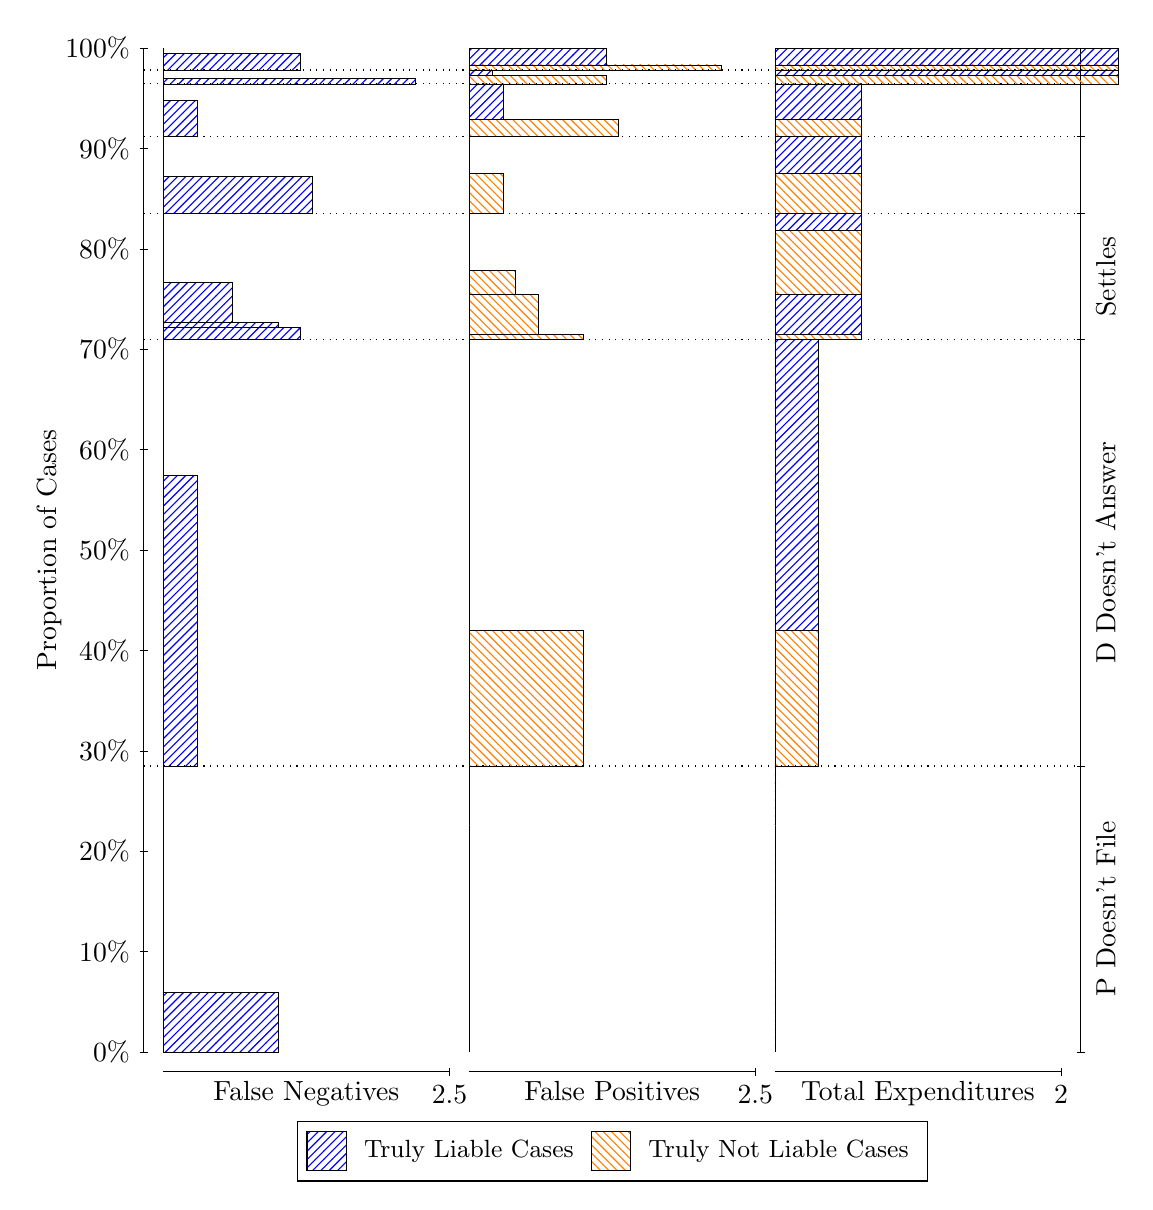
\begin{tikzpicture}
\draw[black, very thin] (1.5,1.75) -- (1.5,14.5);
\node[rotate=90, text=black, anchor=center] at (0.3, 8.125) {Proportion of Cases};
\draw[black, very thin] (1.45,1.75) -- (1.55,1.75);
\node[text=black, anchor=east] at (1.45, 1.75) {0\%};
\draw[black, very thin] (1.45,3.025) -- (1.55,3.025);
\node[text=black, anchor=east] at (1.45, 3.025) {10\%};
\draw[black, very thin] (1.45,4.3) -- (1.55,4.3);
\node[text=black, anchor=east] at (1.45, 4.3) {20\%};
\draw[black, very thin] (1.45,5.575) -- (1.55,5.575);
\node[text=black, anchor=east] at (1.45, 5.575) {30\%};
\draw[black, very thin] (1.45,6.85) -- (1.55,6.85);
\node[text=black, anchor=east] at (1.45, 6.85) {40\%};
\draw[black, very thin] (1.45,8.125) -- (1.55,8.125);
\node[text=black, anchor=east] at (1.45, 8.125) {50\%};
\draw[black, very thin] (1.45,9.4) -- (1.55,9.4);
\node[text=black, anchor=east] at (1.45, 9.4) {60\%};
\draw[black, very thin] (1.45,10.675) -- (1.55,10.675);
\node[text=black, anchor=east] at (1.45, 10.675) {70\%};
\draw[black, very thin] (1.45,11.95) -- (1.55,11.95);
\node[text=black, anchor=east] at (1.45, 11.95) {80\%};
\draw[black, very thin] (1.45,13.225) -- (1.55,13.225);
\node[text=black, anchor=east] at (1.45, 13.225) {90\%};
\draw[black, very thin] (1.45,14.5) -- (1.55,14.5);
\node[text=black, anchor=east] at (1.45, 14.5) {100\%};

\draw[black, very thin] (13.4,1.75) -- (13.4,14.5);
\draw[black, very thin] (13.35,1.75) -- (13.45,1.75);
\node[anchor=west] at (13.35, 1.75) {};
\draw[black, very thin] (13.35,5.3821) -- (13.45,5.3821);
\node[anchor=west] at (13.35, 5.3821) {};
\draw[black, very thin] (13.35,10.801) -- (13.45,10.801);
\node[anchor=west] at (13.35, 10.801) {};
\draw[black, very thin] (13.35,12.398) -- (13.45,12.398);
\node[anchor=west] at (13.35, 12.398) {};
\draw[black, very thin] (13.35,13.376) -- (13.45,13.376);
\node[anchor=west] at (13.35, 13.376) {};
\draw[black, very thin] (13.35,14.044) -- (13.45,14.044);
\node[anchor=west] at (13.35, 14.044) {};
\draw[black, very thin] (13.35,14.221) -- (13.45,14.221);
\node[anchor=west] at (13.35, 14.221) {};
\draw[black, very thin] (13.35,14.5) -- (13.45,14.5);
\node[anchor=west] at (13.35, 14.5) {};

\draw[black, very thin, pattern color=blue, pattern=north east lines] (1.75,1.75) rectangle (3.2033,2.5057);
\draw[black, very thin, pattern color=orange, pattern=north west lines] (1.75,2.5057) rectangle (1.75,5.3821);
\draw[black, very thin, pattern color=blue, pattern=north east lines] (1.75,5.3821) rectangle (2.186,9.0766);
\draw[black, very thin, pattern color=orange, pattern=north west lines] (1.75,9.0766) rectangle (1.75,10.801);
\draw[black, very thin, pattern color=blue, pattern=north east lines] (1.75,10.801) rectangle (3.494,10.952);
\draw[black, very thin, pattern color=blue, pattern=north east lines] (1.75,10.952) rectangle (3.2033,11.012);
\draw[black, very thin, pattern color=blue, pattern=north east lines] (1.75,11.012) rectangle (2.622,11.525);
\draw[black, very thin, pattern color=orange, pattern=north west lines] (1.75,11.525) rectangle (1.75,12.398);
\draw[black, very thin, pattern color=blue, pattern=north east lines] (1.75,12.398) rectangle (3.6393,12.865);
\draw[black, very thin, pattern color=orange, pattern=north west lines] (1.75,12.865) rectangle (1.75,13.376);
\draw[black, very thin, pattern color=blue, pattern=north east lines] (1.75,13.376) rectangle (2.186,13.831);
\draw[black, very thin, pattern color=orange, pattern=north west lines] (1.75,13.831) rectangle (1.75,14.044);
\draw[black, very thin, pattern color=blue, pattern=north east lines] (1.75,14.044) rectangle (4.9473,14.11);
\draw[black, very thin, pattern color=orange, pattern=north west lines] (1.75,14.11) rectangle (1.75,14.221);
\draw[black, very thin, pattern color=blue, pattern=north east lines] (1.75,14.221) rectangle (3.494,14.434);
\draw[black, very thin, pattern color=orange, pattern=north west lines] (1.75,14.434) rectangle (1.75,14.5);
\draw[black, very thin, pattern color=orange, pattern=north west lines] (5.6333,1.75) rectangle (5.6333,4.6263);
\draw[black, very thin, pattern color=blue, pattern=north east lines] (5.6333,4.6263) rectangle (5.6333,5.3821);
\draw[black, very thin, pattern color=orange, pattern=north west lines] (5.6333,5.3821) rectangle (7.0867,7.1066);
\draw[black, very thin, pattern color=blue, pattern=north east lines] (5.6333,7.1066) rectangle (5.6333,10.801);
\draw[black, very thin, pattern color=orange, pattern=north west lines] (5.6333,10.801) rectangle (7.0867,10.861);
\draw[black, very thin, pattern color=orange, pattern=north west lines] (5.6333,10.861) rectangle (6.5053,11.374);
\draw[black, very thin, pattern color=orange, pattern=north west lines] (5.6333,11.374) rectangle (6.2147,11.673);
\draw[black, very thin, pattern color=blue, pattern=north east lines] (5.6333,11.673) rectangle (5.6333,12.398);
\draw[black, very thin, pattern color=orange, pattern=north west lines] (5.6333,12.398) rectangle (6.0693,12.909);
\draw[black, very thin, pattern color=blue, pattern=north east lines] (5.6333,12.909) rectangle (5.6333,13.376);
\draw[black, very thin, pattern color=orange, pattern=north west lines] (5.6333,13.376) rectangle (7.5227,13.589);
\draw[black, very thin, pattern color=blue, pattern=north east lines] (5.6333,13.589) rectangle (6.0693,14.044);
\draw[black, very thin, pattern color=orange, pattern=north west lines] (5.6333,14.044) rectangle (7.3773,14.155);
\draw[black, very thin, pattern color=blue, pattern=north east lines] (5.6333,14.155) rectangle (5.924,14.221);
\draw[black, very thin, pattern color=orange, pattern=north west lines] (5.6333,14.221) rectangle (8.8307,14.287);
\draw[black, very thin, pattern color=blue, pattern=north east lines] (5.6333,14.287) rectangle (7.3773,14.5);
\draw[black, very thin, pattern color=orange, pattern=north west lines] (9.5167,1.75) rectangle (9.5167,4.6263);
\draw[black, very thin, pattern color=blue, pattern=north east lines] (9.5167,4.6263) rectangle (9.5167,5.3821);
\draw[black, very thin, pattern color=orange, pattern=north west lines] (9.5167,5.3821) rectangle (10.062,7.1066);
\draw[black, very thin, pattern color=blue, pattern=north east lines] (9.5167,7.1066) rectangle (10.062,10.801);
\draw[black, very thin, pattern color=orange, pattern=north west lines] (9.5167,10.801) rectangle (10.607,10.861);
\draw[black, very thin, pattern color=blue, pattern=north east lines] (9.5167,10.861) rectangle (10.607,11.374);
\draw[black, very thin, pattern color=orange, pattern=north west lines] (9.5167,11.374) rectangle (10.607,12.187);
\draw[black, very thin, pattern color=blue, pattern=north east lines] (9.5167,12.187) rectangle (10.607,12.398);
\draw[black, very thin, pattern color=orange, pattern=north west lines] (9.5167,12.398) rectangle (10.607,12.909);
\draw[black, very thin, pattern color=blue, pattern=north east lines] (9.5167,12.909) rectangle (10.607,13.376);
\draw[black, very thin, pattern color=orange, pattern=north west lines] (9.5167,13.376) rectangle (10.607,13.589);
\draw[black, very thin, pattern color=blue, pattern=north east lines] (9.5167,13.589) rectangle (10.607,14.044);
\draw[black, very thin, pattern color=orange, pattern=north west lines] (9.5167,14.044) rectangle (13.877,14.155);
\draw[black, very thin, pattern color=blue, pattern=north east lines] (9.5167,14.155) rectangle (13.877,14.221);
\draw[black, very thin, pattern color=orange, pattern=north west lines] (9.5167,14.221) rectangle (13.877,14.287);
\draw[black, very thin, pattern color=blue, pattern=north east lines] (9.5167,14.287) rectangle (13.877,14.5);
\draw[black, dotted] (1.5,5.3821) -- (13.4,5.3821);
\draw[black, dotted] (1.5,10.801) -- (13.4,10.801);
\draw[black, dotted] (1.5,12.398) -- (13.4,12.398);
\draw[black, dotted] (1.5,13.376) -- (13.4,13.376);
\draw[black, dotted] (1.5,14.044) -- (13.4,14.044);
\draw[black, dotted] (1.5,14.221) -- (13.4,14.221);
\draw[black, very thin] (1.75,1.5) -- (5.3833,1.5);
\node[text=black, anchor=north] at (3.5667, 1.5) {False Negatives};
\draw[black, very thin] (5.3833,1.45) -- (5.3833,1.55);
\node[text=black, anchor=north] at (5.3833, 1.45) {2.5};

\draw[black, very thin] (5.6333,1.5) -- (9.2667,1.5);
\node[text=black, anchor=north] at (7.45, 1.5) {False Positives};
\draw[black, very thin] (9.2667,1.45) -- (9.2667,1.55);
\node[text=black, anchor=north] at (9.2667, 1.45) {2.5};

\draw[black, very thin] (9.5167,1.5) -- (13.15,1.5);
\node[text=black, anchor=north] at (11.333, 1.5) {Total Expenditures};
\draw[black, very thin] (13.15,1.45) -- (13.15,1.55);
\node[text=black, anchor=north] at (13.15, 1.45) {2};

\node[text=black, centered, rotate=90] at (13.72, 3.566) {P Doesn't File};
\node[text=black, centered, rotate=90] at (13.72, 8.0916) {D Doesn't Answer};
\node[text=black, centered, rotate=90] at (13.72, 11.599) {Settles};





\draw (7.449999999999999,1.5) node[draw=none] (baseCoordinate) {};
\begin{scope}[align=center]
        \matrix[scale=0.5, draw=black, below=0.5cm of baseCoordinate, nodes={draw}, column sep=0.1cm]{
            \node[rectangle, draw, minimum width=0.5cm, minimum height=0.5cm, pattern color=blue, pattern=north east lines] {}; &
            \node[draw=none, font=\small, text=black] (B) {Truly Liable Cases}; &
            \node[rectangle, draw, minimum width=0.5cm, minimum height=0.5cm, pattern color=orange, pattern=north west lines] {}; &
            \node[draw=none, font=\small, text=black] (B) {Truly Not Liable Cases}; \\
            };
\end{scope}

\end{tikzpicture}
\end{document}